\chapter{Concetti Teorici}
\section{Introduzione}
In questo capitolo vengono illustrati i concetti teorici su cui alcune tecnologie, utilizzate per la realizzazione dell'hello world, si basano.

\section{DevOps}
\subsection{DevOps e Microservizi}
Come discusso nel precedente capitolo, i microservizi sono un approccio architetturale che permette di frammentare il software in sviluppo, in piccole componenti che hanno il compito di fornire una singolà attività. L'approccio DevOps \cite{7458761} fornisce gli strumenti necessari per la gestione, lo sviluppo e la distribuzione delle applicazioni basate sui microservizi.

Data la natura dell'architettura che stiamo presentando non tutte le componenti devono essere sviluppate o integrate da noi, è possibile fare affidamento ai servizi cloud, più in generale si tende a non sviluppare componenti che magari sono già disponibile e pronti all'uso, sia per minimizzare il tempo di sviluppo, sia per concentrare tutte le forze del team sulle componenti principali del software. Fare affidamento ad un servizio cloud permette anche di semplificare la manutenzione della componente che vogliamo integrare nel nostro sistema, perché non è più compito nostro curare il servizio.

Ogni servizio però, mantiene le proprie dipendenze e questo crea un problema di integrazione, grazie alla metodologia DevOps sono stati resi disponibili diversi software per far fronte a questa problematica. Oltre al consueto utilizzo di Git per il controllo della versione, di seguito sono riportati alcuni software più diffusi e più utilizzati in questo ambito \cite{Strumenti_di_DevOps}:

\begin{table}[h]
    \centering
     \begin{tabular}{| c | c |} 
     \hline
     Automazione & \ac*{CI/CD}\\ [0.5ex]
     \hline
     Jenkins & CircleCI \\
     Docker & Bamboo \\
     Puppet & TeamCity \\
     Apache Maven & Travis CI \\
     Gradle & Buddy \\
     \hline
     \end{tabular}
    \caption{Strumenti per l'automazione e CI/CD}
    \label{tab:table1}
\end{table}

\begin{table}[h]
    \centering
     \begin{tabular}{| c | c | c | c |} 
     \hline
     Configurazione & Testing & Monitoraggio\\ [0.5ex]
     \hline
     Chef & Selenium & Nagios \\
     Kubernetes & Tricentis Tosca & Prometheus \\
     Ansible & TestSigma & New Relic \\
     Vagrant & IBM Rational Functional & PagerDuty \\
     Consul & SoapUI & Sensu \\
     Terraform &  & Splunk \\
     & & ELK Stack \\
     \hline
     \end{tabular}
    \caption{Strumenti per la configurazione, testing e monitoraggio}
    \label{tab:table2}
\end{table}


\section{Container Linux}
I Container \cite{Container_Linux} sono una tecnologia già apparsa nei primi anni 2000. Nel sistema operativo FreeBSD era presente una funzione chiamata jail, prigione, ed era uno strumento per isolare una porzione del sistema operativo. Tale tecnologia è stata implementata in GNU/Linux dal 2001 e con le varie implementazioni e le varie migliorie sono nati i container, degli spazi del sistema operativo sicuri e controllati.

In Linux il loro funzionamento viene gestito dai cgroups\footnote{Gruppi di Controllo}, strumenti che operano a livello kernel e che permettono di limitare le risorse utilizzate da un processo o da un gruppo di processi. I gruppi di controllo usano systemd che permette di inizializzare i processi ed isolarli dal resto del sistema operativo.

Attualmente i container sono un approccio utilizzato sia in ambito di sviluppo che in ambito di rilascio e sono nati diversi software per la loro gestione come Linux Container Daemon (comunemente chiamato LXD), Podman e Docker.

\begin{figure}[h]
    \centering
    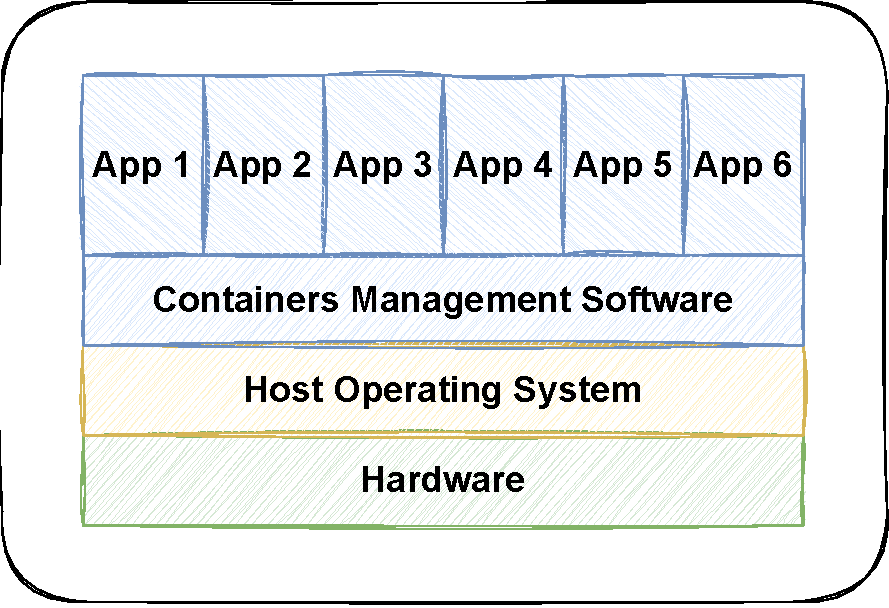
\includegraphics[scale=0.65]{capitoli/immagini/05_container_architecture.pdf}
    \caption{Architettura per la gestione dei container}
    \label{fig:container_architecture}
\end{figure}

\subsection{Macchine Virtuali}
I container vengono molto spesso scambiati per una tipologia di macchina virtuale, questo avviene in maniera errata, perché come abbiamo visto nel paragrafo precedente, i container rappresentano una porzione del sistema operativo creata e gestita da strumenti che lavorano a livello kernel del sistema operativo GNU/Linux. 

Per definizione invece una macchina virtuale crea un ambiante virtuale dove si cerca di emulare il comportamento di una macchina fisica, quindi si cerca non solo di emulare il funzionamento del sistema operativo, ma anche dell'hardware sottostante.

Container e macchine virtuali, seppur diversi per definizione, vengono usati molto spesso per raggiungere lo stesso scopo, quello di rilasciare un software già configurato e pronto all'uso. Per questo motivo ci sono molti lavori che mettono a confronto le due tecnologie come nel caso del lavoro \cite{seo2014performance} di Seo, Kyoung-Taek and Hwang, Hyun-Seo and Moon, Il-Young and Kwon, Oh-Young and Kim, Byeong-Jun che ci permette di osservare come l'utilizzo dei container fornisca delle performance migliori (in questo particolare caso) rispetto all'utilizzo di una macchina virtuale. Questo però non significa che le macchine virtuali ad oggi sono uno strumento datato o superato.

\begin{figure}[h]
    \centering
    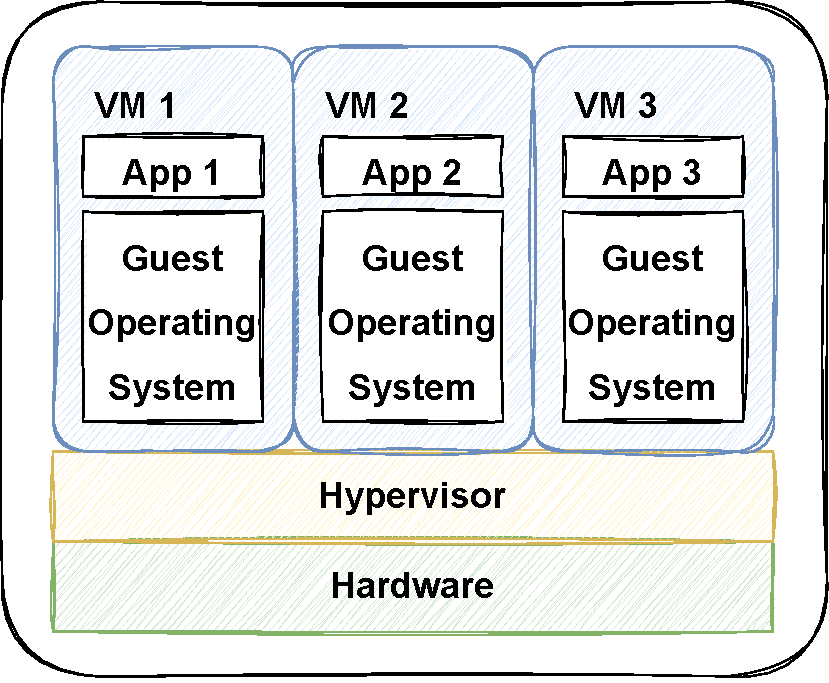
\includegraphics[scale=0.65]{capitoli/immagini/06_virtual_machine_architecture.pdf}
    \caption{Architettura per la gestione di macchine virtuali}
    \label{fig:vm_architecture}
\end{figure}

\subsection{Immagine di un container}
Abbiamo già visto come è definito un container, ora ci chiediamo come sia possibile usare tale tecnologia. I software per la gestione dei container supportano un particolare tipo di file che fornisce agli strumenti che si occupano della creazione del container, importanti schemi di configurazione. Tale file è chiamato immagine di container e rappresenta, in via astratta, quella porzione del sistema operativo che contiene la nostra applicazione con tutte le dipendenze soddisfatte, tutte le configurazioni, gli script e altro.

Le immagini dei container ci permettono di condividere tale applicazioni con altri utenti e di poterle installare con facilità. Ogni programma di gestione dei container definisce il proprio standard di creazione delle immagini.

Di solito le immagini vengono caricate in un  registro, chiamato comunemente container registry, uno spazio dedicato all'archiviazione dell'immagine dove è possibile gestirle ed avere strumenti utili per l'analisi, per esempio alcuni container registry offrono il servizio di analisi delle vulnerabilità.

\subsection{Orchestrazione dei Container}
Ripensando alla definizione data in precedenza per l'architettura a microservizi e applicando a tale definizione la tecnologia appena presentata, possiamo osservare come ogni componente del nostro sistema può essere considerato come un container, in fondo, abbiamo ripetuto più volte che un microservizio è un'entità autonoma e indipendente, e un container, per definizione, è una porzione di sistema operativo isolato (attenzione questo non implica che i container non possano dialogare tra di loro). La nostra applicazione sarà costituita alla fine da tanti container. Data la necessità di dover gestire più container alla volta, sono \cite{burns2022orchestrazione} nati software che si occupano proprio di questo aspetto. 

In generale questo tipo di software creano uno strato aggiuntivo tra l'applicativo che si occupa dei container e i container veri e propri:

\begin{figure}[h]
    \centering
    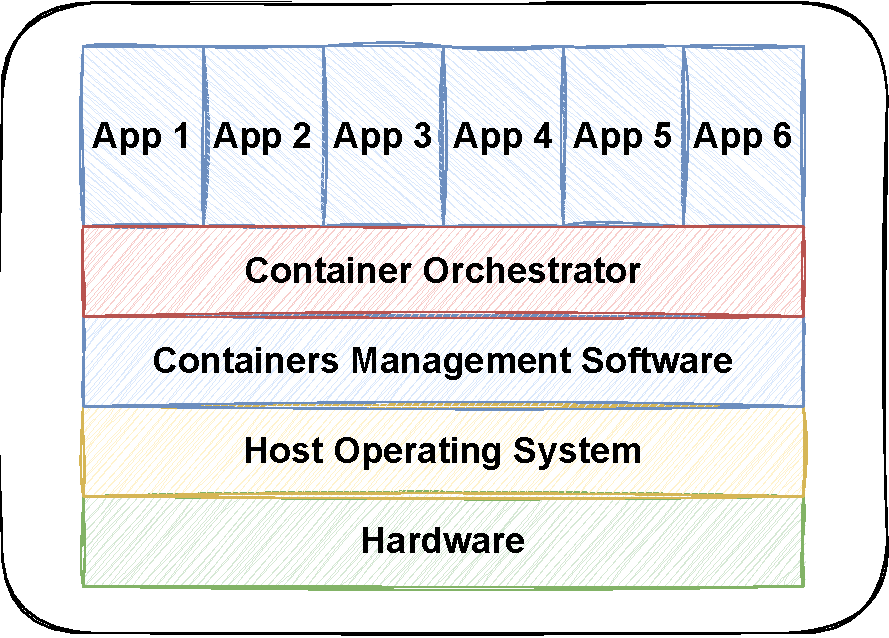
\includegraphics[scale=0.65]{capitoli/immagini/07_container_architecture_orchestrator.pdf}
    \caption{Architettura con software per l'orchestrazione dei container}
    \label{fig:orchestrator}
\end{figure}


Software per l'orchestrazione dei container \cite{cabibbo2022orchestrazione} mettono a disposizione strumenti in grado di eseguire diverse operazioni di gestione, come il monitoraggio dello stato, il carico di lavoro attuale e molto altro.


\section{Lato backend di un applicativo}
Di solito possiamo dividere le nostre applicazioni in due grandi blocchi chiamati rispettivamente backend e frontend. La parte backend di un'applicazione implementa la cosidetta logica di business, mentre la parte di frontend rappresenta ciò che è visibile all'utente finale.

Nel corso degli anni sono nate diverse tecnologie per lo sviluppo e la gestione di questi macro blocchi e con la crescente complessità delle applicazioni sono nati anche dei software utili per gestire e risolvere diversi problemi che appaiono nei grandi progetti, come la gestione delle dipendenze.

Secondo le principali piattaforme di ricerca per il lavoro i linguaggi più popolari per lo sviluppo back end sono: Java, Python, C\# e JavaScript e stanno crescendo l'uso di Rust e Golang.
Di seguito è riportata una tabella con i principali framework assegnati al linguaggio di programmazione:

\begin{table}[h]
    \centering
    \begin{tabular}{| c | c |}
        \hline
       Linguaggio di Programmazione  &  Framework  \\
       \hline
       Java  & Springboot \\
       C\# & ASP.NET \\
       JavaScript & Node.js \\
       Python & Django \\
       \hline
    \end{tabular}
    \caption{Framework associato al proprio linguaggio di programmazione}
    \label{tab:backend_framework}
\end{table}

\subsection{Gestione delle dipendenze}
Una delle problematiche che affligge i gradi progetti è la gestione delle dipendenze. Molto spesso in applicativi reali si tende ad utilizzare diverse tecnologie per rispettare standard o per utilizzare funzioni che il linguaggio di programmazione scelto non rende disponibili tramite le librerie di base. Negli anni sono nati degli strumenti che permettono di automatizzare la gestione delle dipendenze delegando ad un software tutto il lavoro necessario per installare, aggiornare e gestire nuove dipendenze.

\begin{comment}
\subsection{Framework per backend}
Come in ogni altro campo l'avanzamento tecnologico ha portato alla creazione di diverse tecnologie per semplificare lo sviluppo. Anche linguaggi nati principalmente per l'uso in front end hanno visto la creazione di strumenti di framework per lo sviluppo in back end. I linguaggi di programmazione più popolari per lo sviluppo back end secondo le principali piattaforme di ricerca del lavoro sono: Java, Python, C\# e JavaScript e stanno crescendo l'uso di Rust e Golang.

Di seguito è riportata una tabella con i principali framework assegnati al linguaggio di programmazione:

\begin{table}[h]
    \centering
    \begin{tabular}{| c | c |}
        \hline
       Linguaggio di Programmazione  &  Framework  \\
       \hline
       Java  & Springboot \\
       C\# & ASP.NET \\
       JavaScript & Node.js \\
       Python & Django \\
       \hline
    \end{tabular}
    \caption{Framework associato al proprio linguaggio di programmazione}
    \label{tab:backend_framework}
\end{table}
\end{comment}

